\documentclass[11pt, a4paper]{book}
% Ressources à installer : texlive-science et texlive-lang-french ou texlive-lang-european
%à compiler avec XeLaTeX à cause des image pstricks

\usepackage[utf8]{inputenc}
\usepackage[T1]{fontenc}

\usepackage[french]{babel}
\usepackage{listingsutf8}
\usepackage{pdfpages}
\usepackage{tikz,pgf}
\usepackage{amsthm,titlesec}
\usepackage{mdframed} % pour le format des définition, théorèmes...
\usepackage{xcolor,rotating,systeme}
\usepackage[Glenn]{fncychap} %pour le format des chapitres
\usepackage[top=3cm,bottom=3cm,left=3cm,right=2cm,headsep=10pt,a4paper]{geometry} % Page margins
\usepackage{multicol}
\usepackage{comment}
\usepackage{enumerate,cancel}
\usepackage{lipsum,minitoc}
%\usepackage{chngcntr}
\usepackage{amsmath,amsfonts,minitoc,amsthm,pgfplots}
\usepackage{mathrsfs}
\usetikzlibrary{arrows, intersections}
\usepackage{mathrsfs}
\usepackage{array,yhmath}
\usepackage{hyperref}
\usepackage{caption}
\usepackage{float}
\usepackage{wrapfig}
\restylefloat{figure}
%\usepackage{subfig}

\usepackage{subcaption}

\usepackage{listings}
\usepackage{color}
\lstset{ % General setup for the package
    language=Python,
    basicstyle=\footnotesize,
    basewidth=0.7em,
    numbers=left,
     numberstyle=\tiny,
    frame=lines,
    tabsize=4,
    columns=fixed,
    showstringspaces=false,
    showtabs=false,
    keepspaces,
    commentstyle=\color{gray},
    keywordstyle=\color{blue},
    stringstyle=\color{magenta},
    inputencoding=utf8/latin1,
            extendedchars=true,
            literate=%
            {é}{{\'{e}}}1
            {è}{{\`{e}}}1
            {ê}{{\^{e}}}1
            {ë}{{\¨{e}}}1
            {û}{{\^{u}}}1
            {ù}{{\`{u}}}1
            {â}{{\^{a}}}1
            {à}{{\`{a}}}1
            {î}{{\^{i}}}1
            {ô}{{\^{o}}}1
            {ç}{{\c{c}}}1
            {Ç}{{\c{C}}}1
            {É}{{\'{E}}}1
            {Ê}{{\^{E}}}1
            {À}{{\`{A}}}1
            {Â}{{\^{A}}}1
            {Î}{{\^{I}}}1
    }



\usepackage{lipsum}
\newtheorem{example}{Exemple}

\usepackage{pstricks,pst-plot,pstricks-add}
\usepackage{pst-func,tkz-tab,tkz-euclide}
\usepackage{graphicx}
%macro exo
\newcounter{mtex}[chapter]
\newcommand{\mtexlabel}{\cadrexo{\themtex}}
\newcommand{\cadrexo}[1]{%
\tikz\node[rectangle,minimum size=6mm,rounded corners=2mm,fill=ocre,inner sep=0pt,text width=0.8cm,align=center]{\large\bfseries\textcolor{white}{#1}};}
\definecolor{ocre}{RGB}{196,106,106}
\definecolor{vert}{RGB}{55,120,0}
\newcommand{\mtexlabelpos}[1]{%
\makebox[0pt][r]{\raisebox{#1\baselineskip}[0pt][0pt]{\mtexlabel\quad}}}
\newenvironment{exercice}[1][\empty]{%
\refstepcounter{mtex}%
\trivlist\item\relax%  
\ifx#1\empty\mtexlabelpos{-.7}\else\mtexlabelpos{-.5}%
\hfill\textbf{#1}\hfill\mbox{}\par\fi%
}{\endtrivlist}

\newcommand{\N}{\mathbb{N}}
\newcommand{\Z}{\mathbb Z}
\newcommand{\Q}{\mathbb Q}
\newcommand{\R}{\mathbb R}
\newcommand{\C}{\mathbb C}

\newcommand{\ssi}{\;\;\Leftrightarrow\;\;}

\newcommand{\point}[1]{-- +(#1,#1) -- +(-#1,-#1) -- +(0,0) -- +(-#1,#1) -- +(#1,-#1)} 


\newcommand{\parallele}{\mathbin{\!/\mkern-5mu/\!}} %signe parallèle

\titleformat{\chapter}[frame]
{\setlength\fboxrule{2.25pt}\color{black}}%
{\filleft\scshape\LARGE%
\enspace  Chapitre \thechapter\enspace}%
{20pt}
{\rule{0pt}{30pt}\Huge\scshape\filleft}

\newcommand\fonction[5]{
$\begin{array}{rrll}
#1: & #2 & \rightarrow & #3 \\
  & #4 & \mapsto & #5
\end{array}$
}

%\titleformat
%{\section} % command
%[hang] % shape
%{\bfseries\Large} % format
%{ \thesection\quad} % label
%{0em} % sep
%{
%} % before-code
%[
%\vspace{-1ex}%
%\textcolor{blue!60}{\rule{10cm}{3pt}}
%] % after-code


%\theoremstyle{break}
\newtheoremstyle{definition-style}  %style des theoreme
{}               
{}               
{}                   
{}                   
{\bf\sffamily} 
{~:\\[0.3cm]}                 
{.5em}               
{\thmname{#1}\thmnumber{ #2}\thmnote{ (#3)}}

\mdfdefinestyle{defi-frame}{
linewidth=10pt, %
linecolor= blue!50, % 
backgroundcolor= blue!20,
topline=false, %
bottomline=false, %
rightline=false,%
leftmargin=0pt, %
innerleftmargin=15pt, %
innerrightmargin=1em, 
rightmargin=0pt, % 
innertopmargin=-2pt,%
innerbottommargin=6pt, % 
splittopskip=\topskip, %
%splitbottomskip=\topskip, %
}% 

\mdfdefinestyle{methode-frame}{
	linewidth=10pt, %
linecolor= gray!70, % 
backgroundcolor= white,
topline=false, %
bottomline=false,%
rightline=false,%
leftmargin=0pt, %
innerleftmargin=15pt, %
innerrightmargin=1em, 
rightmargin=0pt, % 
innertopmargin=-2pt,%
innerbottommargin=6pt, % 
splittopskip=\topskip, %
%splitbottomskip=\topskip, %
}% 


\mdfdefinestyle{thm-frame}{
linewidth=10pt, %
linecolor= red!50, % 
backgroundcolor= orange!30,
topline=false, %
bottomline=false, %
rightline=false,%
leftmargin=0pt, %
innerleftmargin=15pt, %
innerrightmargin=1em, 
rightmargin=0pt, % 
innertopmargin=-2pt,%
innerbottommargin=6pt, % 
splittopskip=\topskip, %
%splitbottomskip=\topskip, %
}% 

\mdfdefinestyle{lem-frame}{
linewidth=10pt, %
linecolor= yellow!50, % 
backgroundcolor= yellow!10,
topline=false, %
bottomline=false, %
rightline=false,%
leftmargin=0pt, %
innerleftmargin=15pt, %
innerrightmargin=1em, 
rightmargin=0pt, % 
innertopmargin=-2pt,%
innerbottommargin=6pt, % 
splittopskip=\topskip, %
%splitbottomskip=\topskip, %
}% 

\mdfdefinestyle{notation-frame}{
linewidth=10pt, %
linecolor= blue!30, % 
backgroundcolor= blue!10,
topline=false, %
bottomline=false, %
rightline=false,%
leftmargin=0pt, %
innerleftmargin=15pt, %
innerrightmargin=1em, 
rightmargin=0pt, % 
innertopmargin=-2pt,%
innerbottommargin=6pt, % 
splittopskip=\topskip, %
%splitbottomskip=\topskip, %
}% 

\mdfdefinestyle{remarque-frame}{
linewidth=0pt, %
linecolor= black!0, % 
backgroundcolor= blue!0,
topline=false, %
bottomline=false, %
rightline=false,%
leftmargin=0pt, %
innerleftmargin=25pt, %
innerrightmargin=25pt, 
rightmargin=0pt, % 
innertopmargin=-2pt,%
innerbottommargin=6pt, % 
splittopskip=\topskip, %
%splitbottomskip=\topskip, %
}% 
\surroundwithmdframed[style=defi-frame]{defi}

\surroundwithmdframed[style=thm-frame]{thm}

\surroundwithmdframed[style=lem-frame]{lem}

\surroundwithmdframed[style=notation-frame]{notation}

\surroundwithmdframed[style=remarque-frame]{remarque}

\surroundwithmdframed[style=remarque-frame]{remarques}

\surroundwithmdframed[style=methode-frame]{methode}

\theoremstyle{definition-style}

%pour avoir un compteur commun a remarque et remarques
\newcounter{compteurremarque}[chapter]
\renewcommand{\thecompteurremarque}{\arabic{compteurremarque}} %définition de l'affichage du compteur

\newtheorem{defi}{Définition}[chapter]
\renewcommand{\thedefi}{\arabic{defi}} %pour ne pas avoir le numéro du chapitre dans la numération de la def
\newtheorem{thm}{Théorème}[chapter]
\renewcommand{\thethm}{\arabic{thm}}
\newtheorem{lem}{Lemme}[chapter]
\renewcommand{\thelem}{\arabic{lem}}
\newtheorem{notation}{Notation}[chapter]
\renewcommand{\thenotation}{\arabic{notation}}
%\newtheorem{remarque}{Remarque}[chapter]
%\renewcommand{\theremarque}{\arabic{remarque}}
%\newtheorem{remarques}{Remarques}[chapter]
%\renewcommand{\theremarques}{\arabic{remarques}}
\newtheorem{methode}{Méthode}[chapter]
\renewcommand{\themethode}{\arabic{methode}}


\newtheorem{remarque}[compteurremarque]{Remarque}
\newtheorem{remarques}[compteurremarque]{Remarques} %remarque et remarques prennent compteurremarque comme compteur commun

\lstMakeShortInline[columns=fixed]|

%%%%%%%% Commandes de Matthieu

%-------------------------------------------------------------------------------
%---- Eclairage : en encadré sur fond jaune avec symbôle "ampoule" à gauche ----
%-------------------------------------------------------------------------------
\definecolor{coleclairage}{RGB}{255 , 221 , 156}
\definecolor{contoureclairage}{RGB}{255 , 192 , 0}
\newenvironment{eclairage}
{
	\begin{center}%
		\begin{tikzpicture}%
			\node[rectangle, draw=contoureclairage, top color=coleclairage!50, bottom color=coleclairage!140, rounded corners=5pt, inner xsep=5pt, inner ysep=6pt, outer ysep=10pt]\bgroup                     
			\begin{minipage}{0.98\linewidth}
				\begin{minipage}{0.08\linewidth}\centerline{
\includegraphics[scale=1]{images/Symbole_eclairage.png}}\end{minipage}
				\begin{minipage}{0.89\linewidth}\itshape\footnotesize
				}
				{                		
				\end{minipage}
			\end{minipage}\egroup;%
		\end{tikzpicture}%
	\end{center}%
}



\newcommand{\putfigure}[6]{
    \begin{minipage}{#1\textwidth}
    \centering
        \includegraphics[width=#2\textwidth,height=#3\textheight]{#4}
        \captionof{figure}{#5}
        \label{#6}
    \end{minipage}
}


\newcommand{\itemb}[1]{\item \textbf{#1}}



%-------------------------------------------------------------------------------
%---- apprendre : en encadré sur fond jaune avec symbole "ampoule" à gauche ----
%-------------------------------------------------------------------------------
\definecolor{colapprendre}{RGB}{50,205,50}
\definecolor{contourapprendre}{RGB}{34,139,34}
\newenvironment{apprendre}
{
	\begin{center}%
		\begin{tikzpicture}%
			\node[rectangle, draw=contourapprendre, top color=colapprendre!10, bottom color=colapprendre!50, rounded corners=5pt, inner xsep=5pt, inner ysep=6pt, outer ysep=10pt]\bgroup                     
			\begin{minipage}{0.98\linewidth}
				\begin{minipage}{0.08\linewidth}\centerline{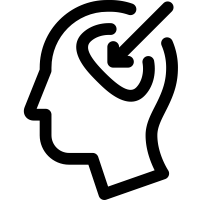
\includegraphics[width=30px]{images/Symbole_learn.png}}\end{minipage}
				\begin{minipage}{0.89\linewidth}\itshape\footnotesize
				}
				{                		
				\end{minipage}
			\end{minipage}\egroup;%
		\end{tikzpicture}%
	\end{center}%
}

\definecolor{colimportant}{RGB}{247 , 189 , 164}
\definecolor{contourimportant}{RGB}{237 , 125 , 49}
\newenvironment{important}
{
	\begin{center}%
		\begin{tikzpicture}%
			\node[rectangle, draw=contourimportant, top color=colimportant!50, bottom color=colimportant!140, rounded corners=5pt, inner xsep=5pt, inner ysep=6pt, outer ysep=10pt]\bgroup                     
			\begin{minipage}{0.08\linewidth}\centerline{
\includegraphics[scale=0.8]{images/Symbole_attention.png}}\end{minipage}
			\begin{minipage}{0.89\linewidth}
			}
			{                		
			\end{minipage}\egroup;
		\end{tikzpicture}%
	\end{center}%
}

%----------------------------------------------
\newcounter{compteurmonprogramme}
\setcounter{compteurmonprogramme}{1}
\newenvironment{monprogramme}
{
	\begin{center}%
		\begin{tikzpicture}%
			\node[rectangle, draw=black, rounded corners=5pt, inner xsep=5pt, inner ysep=6pt, outer ysep=10pt]\bgroup                     
			\begin{minipage}{0.98\linewidth}
				{\bf Programme \thechapter.\thecompteurmonprogramme\;:}
				
				\vspace{2mm}\hspace{7.5mm}
				\begin{minipage}{0.93\linewidth}
				}
				{                		
				\end{minipage}
				\stepcounter{compteurmonprogramme}
			\end{minipage}\egroup;%
		\end{tikzpicture}%
	\end{center}%
}



%------------------------------------------------
%---- Définition : en encadré sur fond blanc ----
%------------------------------------------------
\newcounter{compteurdef}
\setcounter{compteurdef}{1}
\newenvironment{mydefinition}
{
	\begin{center}%
	\begin{tikzpicture}%
		\node[rectangle, draw=black, rounded corners=5pt, inner xsep=5pt, inner ysep=6pt, outer ysep=10pt]\bgroup                    
		\begin{minipage}{0.98\linewidth}
			{\bf {\underline {Définition \thechapter.\thecompteurdef}}}
			
			\vspace{2mm}\hspace{4.5mm}
			\begin{minipage}{0.93\linewidth}
			}
			{                		
			\end{minipage}
			\stepcounter{compteurdef}
		\end{minipage}\egroup;%
	\end{tikzpicture}%
\end{center}%
}

\newenvironment{mydefinitions}
{
	\begin{center}%
		\begin{tikzpicture}%
			\node[rectangle, draw=black, rounded corners=5pt, inner xsep=5pt, inner ysep=6pt, outer ysep=10pt]\bgroup                    
			\begin{minipage}{0.98\linewidth}
				{\bf {\underline {Définitions \thechapter.\thecompteurdef}}}
				
				\vspace{3mm}\hspace{4.5mm}
				\begin{minipage}{0.93\linewidth}\slshape
					\begin{itemize}\setlength{\itemsep}{1mm}
					}
					{                		
				\end{itemize}\end{minipage}
				\stepcounter{compteurdef}
			\end{minipage}\egroup;%
		\end{tikzpicture}%
	\end{center}%
}



%------------------------------------------------
%---- Exemple : en encadré sur fond blanc ----
%------------------------------------------------
\newcounter{compteurex}
\setcounter{compteurex}{1}
\newenvironment{myexample}{
	\begin{center}
	\vspace{-3mm}
	\begin{minipage}{1\linewidth}
		\vspace{2mm}
		{\textsl {\underline {Exemple \thechapter.\thecompteurex}}}
		
		\vspace{2mm}\hspace{2.5mm}
		\begin{minipage}{1\linewidth}
			\begin{mdframed}[topline=false,rightline=false,bottomline=false]
}
{
			\end{mdframed}
		\end{minipage}
		\stepcounter{compteurex}
	\end{minipage}
	\end{center}
}
\newenvironment{myexamples}{
	\begin{center}
		\vspace{-3mm}
		\begin{minipage}{1\linewidth}
			\vspace{2mm}
			{\textsl {\underline {Exemples \thechapter.\thecompteurex}}}
			
			\vspace{2mm}\hspace{2.5mm}
			\begin{minipage}{1\linewidth}%\slshape
				\begin{mdframed}[topline=false,rightline=false,bottomline=false]
					\begin{enumerate}\setlength{\itemsep}{1mm}
				}
				{
					\end{enumerate}
				\end{mdframed}
			\end{minipage}
			\stepcounter{compteurex}
		\end{minipage}
	\end{center}
}



\newtheorem*{question}{Question}



%%%%%%%%%%%%%%%%%%%%%%%%%%%%%%%%%%%%%%%%%%%%%%%%%%%%%%%%%%%%%%%%%%%%%%%%%%%%
%%%%%%%%%%%%%%%%%%%%%%%%%%%   LABELS activite   %%%%%%%%%%%%%%%%%%%%%%%%%%%
%%%%%%%%%%%%%%%%%%%%%%%%%%%%%%%%%%%%%%%%%%%%%%%%%%%%%%%%%%%%%%%%%%%%%%%%%%%%
\newcommand{\act}{\textbf{\textsl{Activité \arabic{compteuract}}} \vspace*{1mm}\\ \addtocounter{compteuract}{1}}
\newcommand{\actnomme}[1]{{\bf Activité \arabic{compteuract} {\textsl{\small (#1)}}}\vspace*{1mm}\\  \addtocounter{compteuract}{1}}
\newcounter{compteuract}
\setcounter{compteuract}{1}
\newcommand{\getactcompteur}{{\the\numexpr \arabic{compteuract} - 1 \relax}}



%%%%%%%%%%%%%%%%%%%%%%%%%%%%%%%%%%%%%%%%%%%%%%%%%%%%%%%%%%%%%%%%%%%%%%%%%%%%
%%%%%%%%%%%%%%%%%%%%%%%%%%%   LABELS EXERCICES   %%%%%%%%%%%%%%%%%%%%%%%%%%%
%%%%%%%%%%%%%%%%%%%%%%%%%%%%%%%%%%%%%%%%%%%%%%%%%%%%%%%%%%%%%%%%%%%%%%%%%%%%
\newcommand{\exo}{\textbf{\textsl{Exercice \arabic{compteurexo}}} \vspace*{1mm}\\ \addtocounter{compteurexo}{1}}
\newcommand{\exonomme}[1]{{\bf Exercice \arabic{compteurexo} {\textsl{\small (#1)}}}\vspace*{1mm}\\  \addtocounter{compteurexo}{1}}
\newcommand{\eexo}{\vspace{5mm}} % espace pour séparer les exercices
\newcounter{compteurexo}
\setcounter{compteurexo}{1}
\newcommand{\getexocompteur}{{\the\numexpr \arabic{compteurexo} - 1 \relax}}
\usepackage{minted}
\pgfplotsset{compat=1.17}
\begin{document}

\setcounter{chapter}{3}


\chapter{Stockage de données}
\section{Introduction}

Les besoins en stockage de données numériques, à l’échelle mondiale, ont été multiplié par plus de vingt au cours de la dernière décennie et devraient dépasser les 50 zettaoctets (1021) d’ici fin 2021. Comme le montre l’infographie ci-dessous, cette quantité de données apparaît finalement dérisoire en comparaison avec ce qui est attendu pour les quinze prochaines années. Les prévisions tablent en effet sur une multiplication par trois ou quatre du volume annuel de données créées tous les cinq ans. Avec ce rythme exponentiel de croissance, le seuil astronomique des 2’000 zettaoctets devrait être franchi à l’horizon 2035.

\begin{figure}[ht!]
\centering
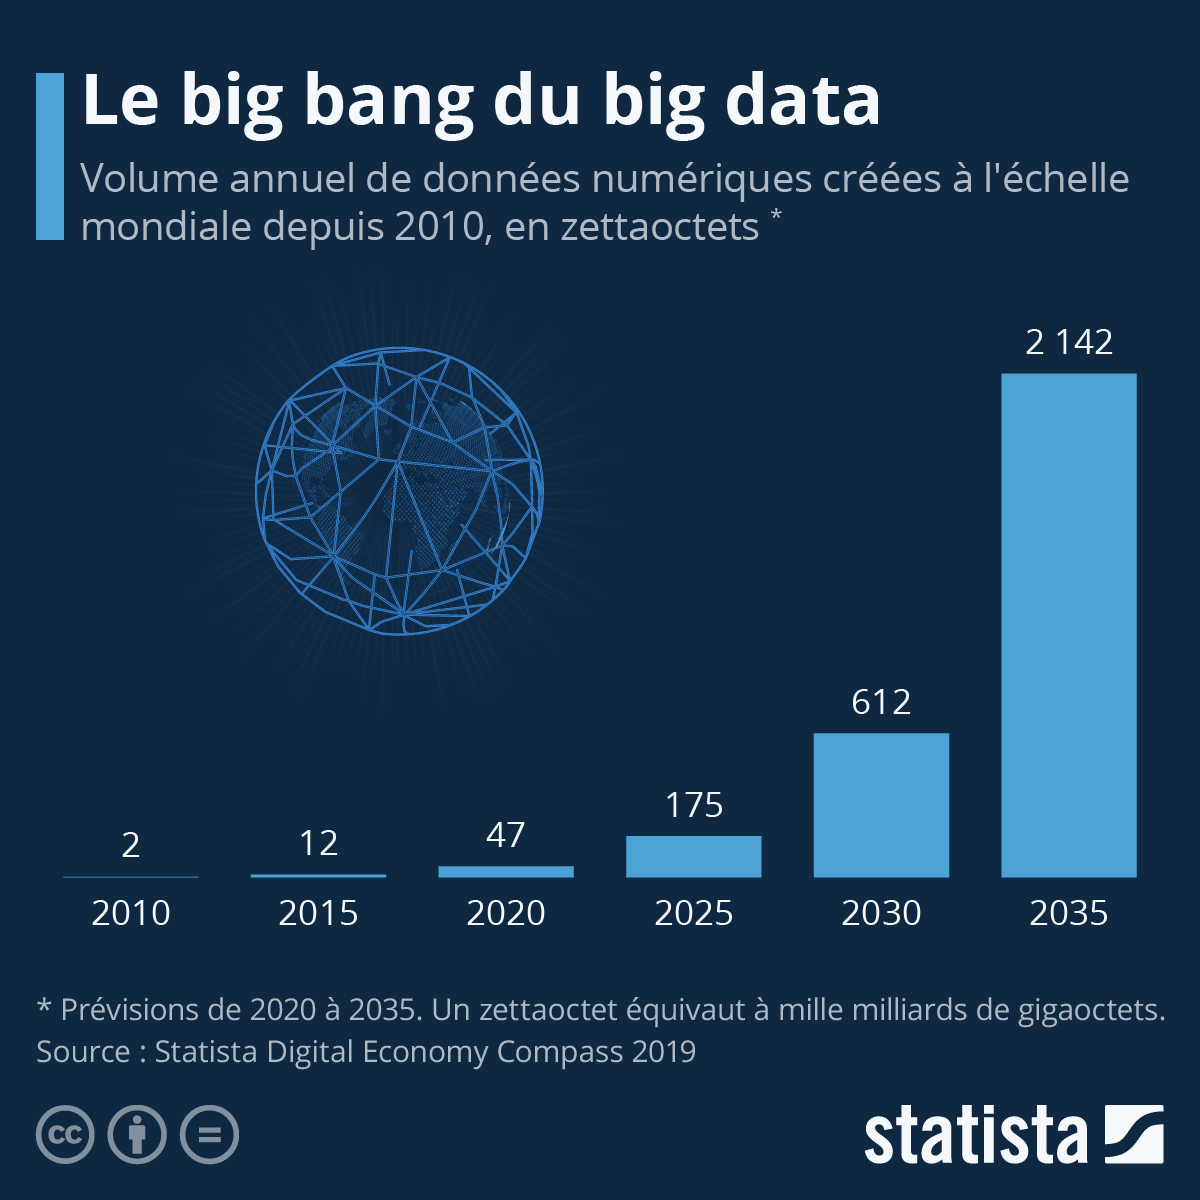
\includegraphics[width=8cm]{images/statista.jpeg}
\end{figure}

Il faudrait se procurer 500 millions de disques durs actuels (100 To) pour être capable de sauvegarder 50 [Zo] ! Cette quantité de données pose autant de problèmes de préservation et d’intégrité des données que de sauvegarde. Sans annoncer les problèmes de places, de consommation électrique, de pollutions dues à la fabrication et au recyclage du matériel vieillissant, de coût et de sauvegarde.

\section{Octet : unités de mesure en informatique}
Rappel : un octet permet de représenter $2^8$ nombres, soit 256 valeurs différentes.
\begin{center}
   \begin{tabular}{| r || c |  c | c | c | c | c | c |  c |}
     \hline
     Symbole & ko & Mo & Go & To & Po & Eo & Zo & Yo \\ \hline
     Nom & kilooctet & mégaoctet & gigaoctet & téraoctet & pétaoctet & exaoctet & zettaoctet & yottaoctet   \\ \hline
     Valeur & $10^{3}$ & $10^{6}$ & $10^{9}$ & $10^{12}$ & $10^{15}$ & $10^{18}$ & $10^{21}$ & $10^{24}$  \\ \hline
   \end{tabular}
\end{center}

Exemples de tailles de fichier (ordre de grandeur):
\begin{enumerate}
    \item[-] 2 Ko :        fichier texte (2’000 lignes de texte)
    \item[-] 1 à 20 Mo :    photo compressée (jpeg) d’un appareil photo numérique.
    \item[-] 10 Mo :     fichier MP3 d’une durée ~5 min (débit 320 kbit/s)
    \item[-] 700 Mo :     film ~1h30 (compression – qualité DVD)
    \item[-] 3 Go :         film ~1h30 (compression – qualité Blu-ray)
    \item[-] 25 Go :     film Blu-ray
\end{enumerate}

\begin{remarque}
Jusqu'en 1998, 1024 octets valaient 1 kilooctet. Puis, les unités ont été standardisées par l'organisme international IEC comme indiqué ci-dessus. On continue cependant à utiliser encore souvent des puissances de 2, tout en changeant l'unité :

Un kilooctet (ko) devrait en principe valoir 1000 octets, mais les ordinateurs utilisent en pratique $2^{10}=1024$ octets, qu'on appelle kibioctets(kio)... ce qui fait une différence de 2.4 \% ! Et on fait de même pour les préfixes suivants : $1 Mio = 2^{20}=1'048'576'$, Mio, Gio, Tio, etc.
\end{remarque}

\section{Support de données}

Quel que soit le type de support, sa taille et son emplacement (local ou distant), ils ont tous certains points communs, comme :
\begin{enumerate}
\item Les supports contiennent des 1 et des 0 qu’il s’agisse de votre dernier livre ou de votre musique préférée.
\item Tous les supports ont un schéma d’organisation des données qui est dépendante du système d’exploitation.
\item Ils ont tous besoin d’être alimentés électriquement pour fonctionner.
\item Aucun support n’est fiable à 100 \% !
\end{enumerate}

\subsection{Supports amovibles}
Avant d’avoir les clés USB et les cartes mémoires que l’on retrouve dans les téléphones mobiles et les appareils photo, il existait d’autres supports externes. Parmi les premiers supports de données informatiques grand public se trouvait la disquette.

\begin{figure}[ht!]
\centering
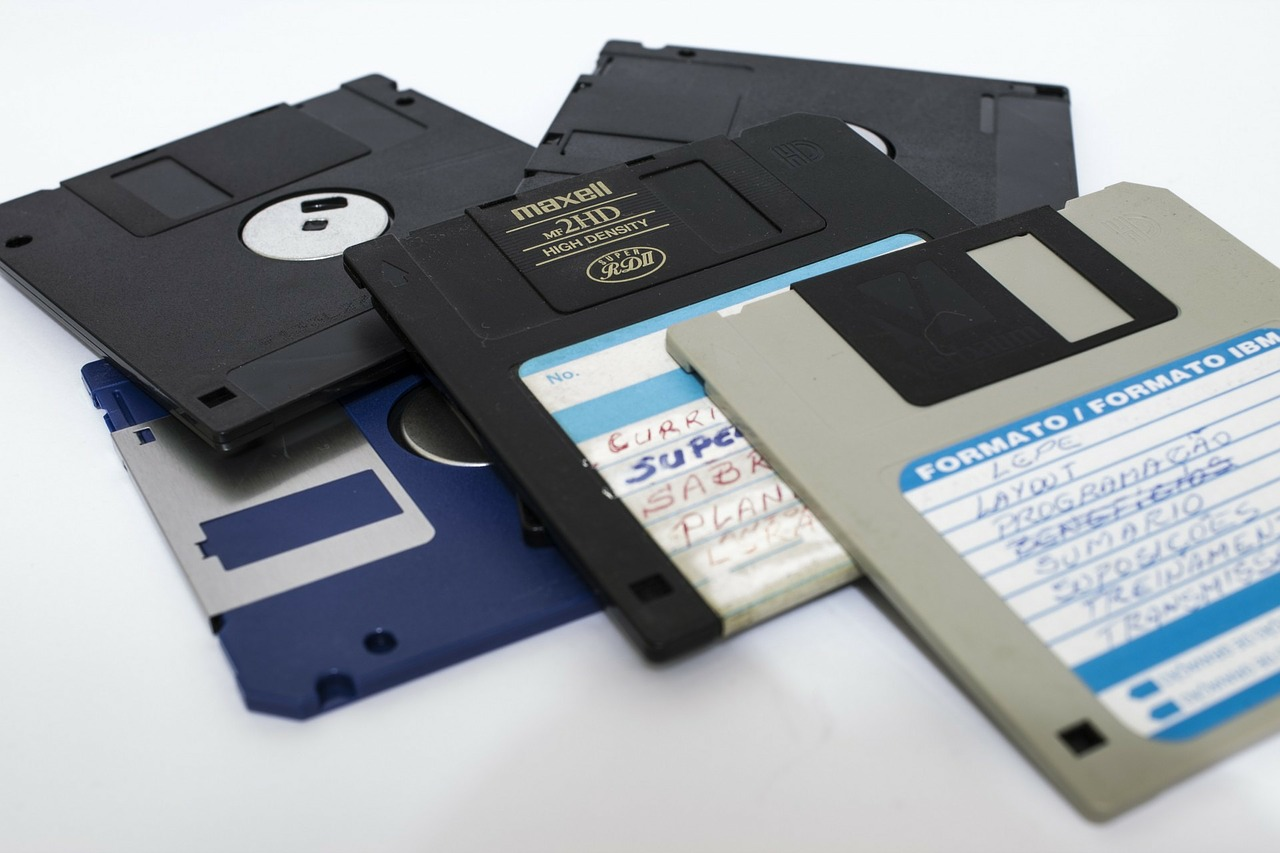
\includegraphics[width=8cm]{images/floppy-disk.jpg}
\end{figure}

Inventée dans les années 1970, elle remplaçait les cartes perforées. Quelques exemples de supports amovibles :
\begin{enumerate}
\item[] 1970 : disquette 8’’ : 1,2 Mo
\item[] 1970 : disquette 5,25’’ 360k
\item[] 1980 : disquette 3,5’’: 1,44 Mo, le standard pendant 20 ans !
\item[] 1990 : CD-ROM 700Mo (d’autre déclinaison jusqu’à 800Mo)
\item[] 1990 : ZIP : 700Mo
\item[] 2004 : DVD-ROM : 4,7 Go
\item[] 2004 : DVD-ROM double couche : 9,4 Go
\item[] 2006 : Blu-ray 25Go
\item[] 2006 : Blu-ray double couche 50Go
\item[] 2000 : clé USB et carte mémoire
\end{enumerate}

\subsection{Supports distants}
Depuis 2010, plusieurs entreprises offrent un service de stockage et de partage de fichiers dans le cloud (ou nuage). Il est donc nécessaire d’avoir une connexion Internet pour accéder à ces espaces de stockage.

\begin{remarques}
Le terme « cloud » est une forme abrégée de « cloud computing » ou l’informatique en nuage. Un cloud est constitué de serveurs situés à distance et accessibles de n’importe où et à n’importe quel moment via une connexion Internet sécurisée et protégée.
\end{remarques}

\begin{figure}[ht!]
\centering
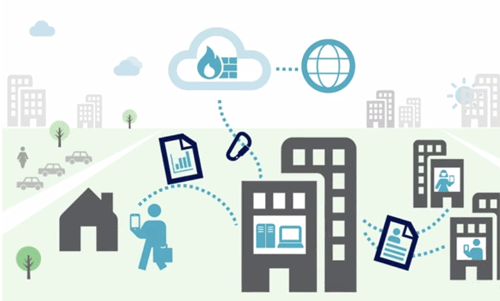
\includegraphics[width=8cm]{images/Business_Network_Solutions_swisscom.png}
\end{figure}

Quels sont les avantages et les inconvénients d’avoir ses données dans un cloud qui ne vous appartient pas (dont vous ne gérez pas l’infrastructure) ?

\begin{example} Vous prenez un contrat chez l’entreprise Tartempion 5 chf par mois pour 1 To de place pour vos données.
\end{example}

\textbf{Avantages principaux du cloud :}
\begin{enumerate}
\item[+] Vos données sont accessibles partout, à condition d’être connecté à Internet. Vos données sont donc accessibles depuis votre smartphone, votre PC, etc.
\item[+] Possibilité de partager ses données. De plus, certains logiciels permettent la modification simultanée et gèrent l’accès concurrent.
\item[+] Aucun investissement ni installation préalable requise, juste le prix de l’abonnement. Il vous suffit en général d’un navigateur web pour accéder à vos données.
\item[+] Maintenance, sécurisation des données et mises à jour effectuées par le fournisseur.
\item[+] Souplesse dans l’espace loué. Si vous avez besoin de 2 To, vous pourrez évoluer votre abonnement.
\item[+] En cas de panne de votre ordinateur personnel, vous ne perdez pas les données qui sont dans le cloud.
\end{enumerate}
\textbf{Inconvénients principaux du cloud :}
\begin{enumerate}
\item[-] Pas de contrôle total d’accès aux données par rapport à l’entreprise Tartempion. Confidentialité des données compromise si aucun outil n’est mis en place pour protéger les documents sensibles ;
\item[-] Savez-vous où sont réellement hébergées vos données ?
\item[-] Dépendance avec l’entreprise. Si Tartempion fait faillite que se passe-t-il ?
\item[-] Risque de cyberattaques si les données ne sont pas bien protégées.
\item[-] Obligation d’être connecté à Internet. Le service peut être dégradé si la liaison n’est pas fiable.
\item[-] Accès aux fichiers plus lents que sur un support local.
\item[-] Impact écologique : par ses serveurs nécessaires au fonctionnement du cloud, ce dernier induit une consommation d’énergie croissante.

\end{enumerate}

\section{Stratégie de sauvegarde}
\subsection{Introduction}
Aucun support de stockage n’a une durée de vie illimitée et aucun support de stockage n’est fiable à 100\%. Le risque zéro n’existe pas. Une perte de données numériques est donc très vite arrivée. Les causes principales sont:
\begin{enumerate}
\item[o] des défaillances techniques matérielles comme un disque dur en panne ou une clé usb qui n’est plus accessible;
\item[o] des défaillances logicielles comme un fichier corrompu suite à une écriture erronée par le système d’exploitation, une erreur de synchronisation;
\item[o] des défaillances humaines comme un fichier effacé, un fichier écrasé ou une clé usb perdue;
\item[o] des catastrophes naturelles comme des incendies ou des dégâts des eaux;
\item[o] des programmes malveillants et des attaques de virus ou de ransomware;
\item[o] le vol du matériel comme votre téléphone portable, un disque d’un serveur, une clé usb, une carte mémoire;
\end{enumerate}
Le monde professionnel indique une durée de vie moyenne de 5 ans pour un disque dur mécanique ou un disque type SSD. Une clé usb ou une carte mémoire de qualité pourrait tenir 10 ans. Le cloud offert par les entreprises de stockage a une durée de vie quasi illimitée, du moins celle de l’entreprise.

\subsection{Stratégie 3-2-1 de sauvegarde de données}

La stratégie de sauvegarde 3-2-1 représente le b-a-ba et le minimum de la protection des données. Mise au point par un photographe souhaitant protéger ses clichés dans les années 1920, cette stratégie est devenue une référence, car elle permet une protection optimale des données, quel que soit leur format.

Le concept de base de la stratégie 3-2-1 repose sur trois principes :
\begin{enumerate}
    \item[->] \textbf{{\huge 3} copies de vos données:} La stratégie recommande d’avoir 2 copies plus la source. Avec trois copies dont deux sauvegardes, le risque que les trois copies aient un problème en même temps est très faible surtout si elles sont stockées sur des supports différents.

    \item[->] \textbf{{\huge 2} supports différents:} La notion de supports différents est essentielle quand on parle de données numériques, car quel est l’intérêt d’avoir deux sauvegardes si elles sont stockées sur le même support ? En cas d’incident, toutes les données seraient perdues. Il est donc important que la source et au moins une de ses copies soient sauvegardées sur des supports différents.

    \item[->] \textbf{{\huge 1} copie hors site:} Quel que soit le support (NAS, disque dur externe, lecteur de bande, etc.), aucune stratégie de sauvegarde de données numériques ne peut être considérée comme sûre si au moins une des copies n’est pas stockée « hors site ». Le récent incendie du 10 mars 2021 d’OVH en est la preuve. En effet, certains utilisateurs avaient leur site en production sur un serveur et leurs copies sur un autre serveur. Certes, les copies étaient sur des supports différents, mais elles étaient stockées dans le même datacenter. Comme une grande partie du site contenant ces serveurs a cessé de fonctionner à cause de l’incendie, aucune des copies n’était utilisable. Or, si au moins une de ces copies avait été stockée chez un autre hébergeur (hors site), ces utilisateurs auraient pu rétablir rapidement leurs services.
\end{enumerate}

Malgré tout les stratégies de sauvegarde ont leurs limites ! La quantité de données à sauvegarder peut prendre trop de temps et poser des problèmes d’intégrité des données. L’externalisation des sauvegardes selon la méthode 3-2-1 soulève aussi la question de la protection des données. 

Et si vous avez bien conservé votre donnée numérique. Serez-vous capable de la relire ?

\section{Exercices}

\begin{exercice}
En réfléchissant aux derniers cours, essayez de calculez la taille que ferait un fichier texte \texttt{blabla.txt} contentant la chaîne de caractères \texttt{blablabla}.
Vérifiez ensuite en le créant sur votre ordinateur.
\end{exercice}


\begin{exercice}
Reprenez le dossier \texttt{Nourriture} de l'exercice 2 du chapitre précédent. Compressez-le et comparez sa taille originale avec sa taille une fois compressé.
\end{exercice}

\begin{exercice}
Téléchargez l'image \texttt{sample\_1920x1280.bmp} en haute définition depuis moodle puis convertissez-la dans les formats suivants en comparant la taille et la qualité de l'image à chaque étape. 

\textit{Utilisez par exemple le site \url{https://online-converting.com/image} pour faire la conversion en jpg et \url{https://online-converting.com/image/convert2bmp} pour le bmp}
\begin{center}
   \begin{tabular}{| l || c | r | }
     \hline
     Format & Taille (ko) & Qualité visuelle \\ \hline
     .bmp en 24 bits &  &  \\ \hline
     .bmp en 8 bits &  &  \\ \hline
     .jpg &  &  \\ \hline
     .png &  &  \\
     \hline
   \end{tabular}
\end{center}
\end{exercice}

\end{document}